% !TeX root = ../main.tex

\chapter{风云四号云图雷暴提取}
第二章分析了卫星云图特征提取中几种常用的特征,本章则针对风云四号卫星云图数据,从传感器波段选择、
雷暴尺度强度以及特征融合等三个方面,分析雷暴提取中可能涉及到的相关问题。

\section{传感器波段问题}
地球被大气圈所包围,离地面越高,大气越稀薄。按大气温度的垂直结构,可把大气圈分为对流层、
平流层、中间层和热层,如图3.1所示。

\begin{figure}[htb]
    \centering
    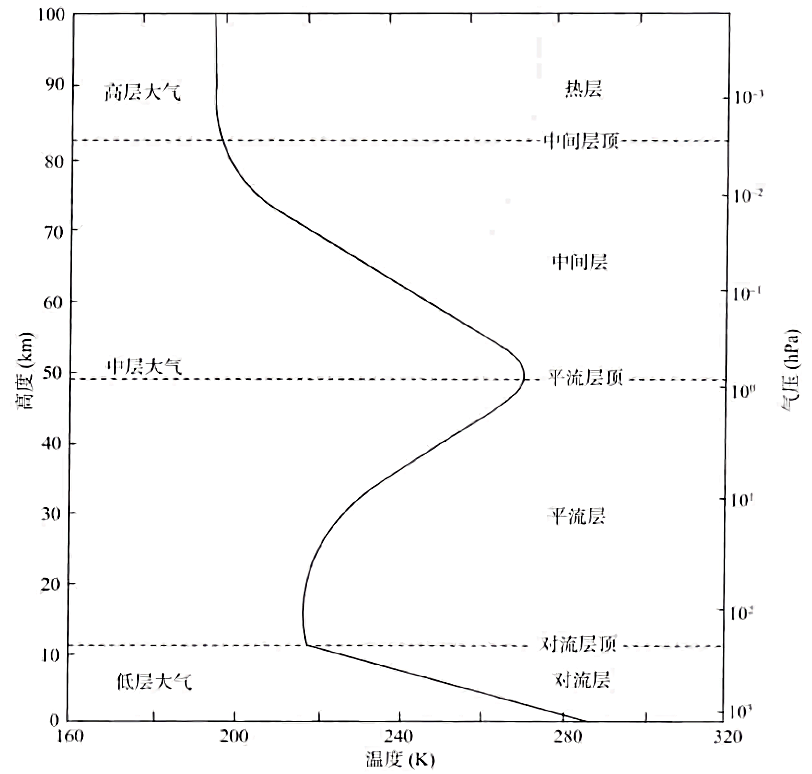
\includegraphics[height=0.9\textwidth]{大气垂直温度轮廓线和分层1.png}
    \caption{大气垂直温度轮廓线和分层}
    %\label{fig:logo}
    %\note{注:图注的内容不宜放到图题中。}
\end{figure}
地面以上大气的最底层称为对流层,对流层顶的高度约为10km,气压约为200hPa。
对流层集中了大气质量的75$\%$
以上,几乎全部云、水汽和降水,主要天气现象,如台风、寒潮和雷电等,都发生在这层。
温度随高度升高而降低是对流层的主要特征,大约每升高1 km降低6.5$^\circ C$。

对流层顶向上到50km左右的这一层为平流层,平流层顶的气压约为1 hPa。 
平流层下部温度随高度变化很小,平流层上部因为存在臭氧层,
臭氧吸收太阳紫外辐射使大气温度增加,这种上部热下部冷的逆温结构平流层大气很稳定,
空气大多做水平运动。
平流层顶到85 km左右称为中间层,中间层顶气压约0.01 hPa,中间层大气温度随高度递减,
水汽极少,有相当强的垂直混合,60 km以上大气分子开始电离,电离层的底部就在中间层内。
中间层顶以上到500 km的这一层称为热层。由于热层的分子氧和原子氧能吸收太阳紫外辐射和微粒辐射,
所以这一层温度又随高度升高而增加,很难有对流运动,造成巨大温度梯度和昼夜温差。

在构成大气的气体中,氮气($N_2$)和氧气($O_2$)约占99$\%$,
氩气($Ar$)、水汽($H_20$)、二氧化碳($CO_2$)、臭氧($O_3$)及其他气体($H_20$,$CH_4$,$NH_4$等)约占1$\%$,
图3.2给出了主要吸收气体的垂直分布廓线。大气中还包含各种气溶胶等微粒。
气溶胶是一种固体、液体的悬浮物,由尘埃、盐粒等组成一个核心,在核心以外包有一层液体。

\begin{figure}[htb]
    \centering
    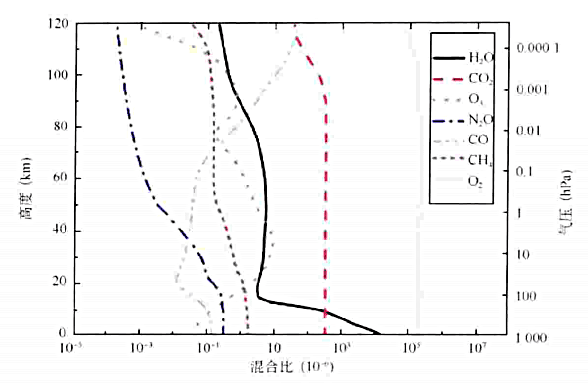
\includegraphics[height=0.6\textwidth]{不同气体的垂直分布廓线1.png}
    \caption{不同气体的垂直分布廓线}
    %\label{fig:logo}
    %\note{注:图注的内容不宜放到图题中。}
\end{figure}

气体分子对不同波长的辐射有强烈而复杂的吸收光谱,图3.3为主要吸收气体的光谱分布图。
对流层中,水汽是最重要的吸收气体,其次是$CO_2$;平流层中,$H_20$,$CO_2$和$0_3$的吸收作用相当;
中间层大气中的主要吸收气体是$CO_2$。

\begin{figure}[htb]
    \centering
    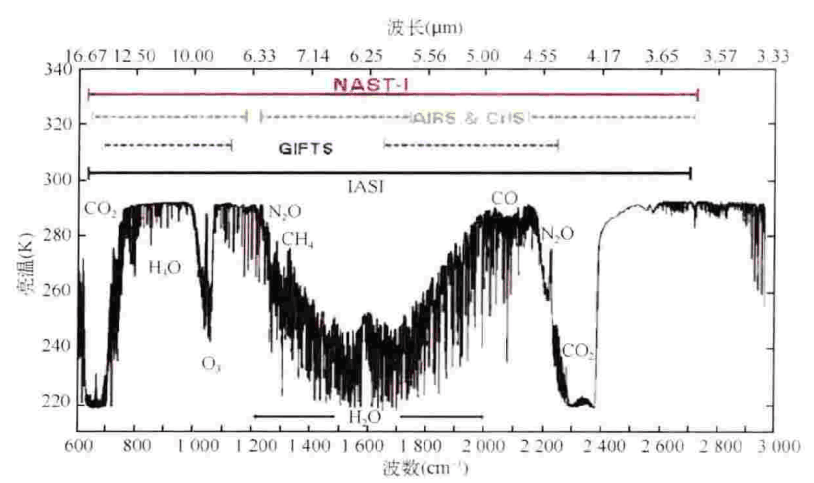
\includegraphics[width=\textwidth]{不同气体的吸收光谱.png}
    \caption{不同气体的吸收光谱}
    %\label{fig:logo}
    %\note{注:图注的内容不宜放到图题中。}
\end{figure}

多通道扫描成像辐射计是风云四号的载荷之一,
通过精密的双扫描镜机构实现灵活和精确的二维指向,
可实现分钟级的快速区域扫描;采用离轴三反主光学系统,高频次获取十四波段的地球云图,
利用星上黑体,进行高频次红外定标,确保了观测数据的精度\cite{FY4A}。

多通道扫描成像辐射计主要负责获取云图的任务,共十四个通道,是风云二号五通道的近三倍,
在风云二号观测水汽、云、地表和植被的基础上,还具备了捕捉雪和气溶胶的能力,
并且能清晰区分云的不同相态和中高层水汽。与风云二号单一可见光通道相比,
风云四号可以制作出彩色卫星云图,1分钟即可生成一次区域观测图像。成像仪的主要技术指标如表3.1所示。

\begin{table}[htb]
    \centering\small
    \caption{多通道扫描辐射计主要技术指标}
    \label{tab:exampletable}
    \begin{tabular}{ll}
      \toprule
        技术指标   & 指标参数     \\
      \midrule
      搭载卫星 & FY-4A \\
      重量 & 306Kg   \\
      通道数量 & 14个(6个可见/近红外波段,2个中波红外波段, \\
       & 2个水汽波段和4个长波红外波段)       \\
      空间分辨率 & 可见/近红外波段为0.5$\sim$1Km,红外波段为2Km$\sim$4Km     \\
      全圆盘扫描时间 & 15分钟  \\
      区域扫描时间 & 1分钟(1000Km$\times$1000Km)  \\
      \bottomrule
    \end{tabular}
  \end{table}

  \begin{table}[htb]
    \centering\small
    \caption{多通道扫描辐射计主要技术指标}
    \label{tab:exampletable}
    \begin{tabular}{cllll}
      \toprule
        通道序号 & 通道类型 & 中心波长  & 空间分辨率 & 主要用途    \\
      \midrule
      1 & 可见光与近红外 & $0.45\mu m$  & 1Km & 小粒子气溶胶 \\
      2 &  & 0.65$\mu m$ & 0.5Km$\sim$1Km & 植被 \\
      3 &  & 0.82$\mu m$ &  1Km & 植被,水面上气溶胶 \\
      4 & 短波红外 & 1.37$\mu m$ & 2Km & 卷云 \\
      5 &  & 1.61$\mu m$  & 2Km & 低云/雪识别 \\
      6 &  & 2.25$\mu m$ & 2Km$\sim$4Km & 卷云、气溶胶 \\
      7 & 中波红外 & 3.75$\mu m$ & 2Km & 云等高反照率目标 \\
      8 &  & 3.75$\mu m$ & 4Km & 低反照率目标,地表 \\
      9 & 水汽 & 6.25$\mu m$  & 4Km & 高层水汽 \\
      10 &  & 7.1$\mu m$  & 4Km & 中层水汽 \\
      11 & 长波红外 & 8.5$\mu m$  & 4Km & 总水汽\\
      12 &  & 10.7$\mu m$  & 4Km & 云、地表温度等 \\
      13 &  & 12.0$\mu m$  & 4Km & 云、总水汽量\\
      14 &  & 13.5$\mu m$ & 4Km & 云、水汽 \\
      \bottomrule
    \end{tabular}
  \end{table}
  
成像仪各通道性能参数如表3.2所示。可以观察到,序号低的通道(波长短)主要观测近地气溶胶及低云,
序号高的通道(波长长)主要观测中高层水汽。根据雷暴云的物理特性,雷暴成熟时云顶高度高,中高层云聚集大量水汽,
可知在中长波红外和水汽通道能够较好反映出雷暴信息。


\section{雷暴尺度及强度问题}
雷暴是由强对流生成的,
由水平尺度几千米到十几千米的雷暴单体的积雨云所组成,有雷电活动的单体寿命约为30分钟到1小时。
闪电率可以从每分钟不足一次到每分钟十次以上,通常在第一次闪电之后大约10$\sim$20 min内出现最大的闪电。
在单体整个生存期内,平均闪电率约为每分钟2至3次,但是雷暴是由多个单体组成,对整个雷暴而言,
平均闪电率约为每分钟3至4次。

本文所采用的风云四号数据为成像仪全圆盘4KML1级数据,该数据包含扫描辐射成像计14个通道的云图信息,
云图分辨率为4km。在建立样本库时,将会从不同通道提取出不同宽度的正方形云图,
根据雷暴云的物理特性,可以计算出样本库单个云图应取50个像素值左右,若取值过多,则超过雷暴云的尺度范围,
将会包含更多无效信息;若取值过少,将无法提取出雷暴云的图像特征。

风云四号的闪电数据由卫星上搭载的闪电成像仪提供,闪电成像仪采用CCD面阵和光学成像技术,
对观测区域内包括云闪、云地闪和云间闪在内的总闪电进行凝视观测,实现对雷暴系统的实时、
连续监测和跟踪,为强对流天气监测、铁路、电力和民航等行业安全保障等提供服务\cite{fengyunsihao}。
闪电成像仪主要技术指标如表3.3所示。

\begin{table}[htb]
    \centering\small
    \caption{闪电成像仪主要技术指标}
    \label{tab:exampletable}
    \begin{tabular}{ll}
      \toprule
        技术指标   & 指标参数     \\
      \midrule
      搭载卫星 & FY-4A \\
      重量 & 65Kg   \\
      尺寸 &  528mm(长)$\times$346mm(宽)$\times$1032mm(高)\\
      CCD面阵 &  400$\times$600单元\\
      成像速率 & 500帧/秒  \\
      中心波长 & 777.4nm \\
      带宽 & 1nm \\
      空间分辨率 & 7.8Km@星下点 \\
      总视场角 & 4.98$\circ$(南北)$\times$7.41$\circ$(东西)\\
      闪电探测率 & 90$\%$  \\
      虚警率 & 10$\%$ \\
      \bottomrule
    \end{tabular}
  \end{table}

闪电成像仪 CCD 面阵利用 777.4 nm近红外通道探测发光事件,经星上实时事件处理器进行背景光评估,输出经背景光
滤除后的发光事件的强度和位置等信息,通过聚类滤除算法将发光事件聚类为“事件”,“组”和“闪电”产品,
包括“事件”,“组”和“闪电”的位置、强度和发生时间等信息。处理过后以闪电仪1分钟组产品的方式发送给用户,
该产品为NC格式的数据,存储有“闪电组”的经纬度,时间,强度等信息,其中GEC(Group Event Count)
存储了闪电的强度信息,闪电强度越大,对应位置的雷暴云图特征将更为明显\cite{lmi}\cite{shandianyi}。


\section{特征融合问题}
本文选用灰度共生矩阵的方法计算出角二阶矩、对比度、逆差距和熵等四种纹理特征量化值,几何特征方面选取了云区
面积、质心、偏心率等特征,数据分析中多维的数据往往很难找出准确的特征,
因此本文将采用主成分分析的方法来分析和简化数据。

在多元统计分析中,主成分分析(Principal components analysis,PCA)
可以用来降低数据集的维数,同时保留数据集中对方差贡献最大的特征。
这是通过忽略高阶主成分,保留低阶主成分做到的,
由于主成分分析过于依赖所给数据,所以对数据的准确性要求很高。

主成分分析由卡尔·皮尔逊于1901年发明,用于建立数理模型和分析数据。
其方法主要是通过对协方差矩阵进行特征分解,以得出数据的主成分(即特征向量)与它们的权值(即特征值)。
PCA是最简单的以特征量分析多元统计分布的方法。 结果可以理解为数据值对方差影响最大的方向。
PCA提供了一种减少数据维度的有效方法,如果从原始数据中移除对应于最小特征值的分量,
所得到的低维数据就是优化过的,在分析复杂数据时,主成分分析特别有用。

PCA是以特征量分析多元数据统计分布的方法。通常情况下,这种运算可以被看作是一种揭露数据的内部结构,
从而更好的解释数据变量的方法。如果多元数据集能够在一个高维数据空间坐标系中被表示出来,
那么PCA就能够计算出一幅比较低维度的图像,这幅图像即为在信息最多的点上原对象的一个‘投影’。
这样就可以利用少量的主成分来降低数据的维度。

遥感图像处理中一幅多波段遥感图像的不同波段之间往往存在着很高的相关性,
对其进行主成分变换的实质是将具有相关性的多波段数据压缩到完全独立的较少的几个波段上,
使新图像数据更易于解译。将不同时相的多波段数据经主成分变换后,
新图像中各主分量正交即各主分量之间的相关系数为零或接近零。
一般来说,第一主分量包括了原始多波段影像信息的绝大部分内容,相当于原来各波段的加权和,
每个波段的权值与该波段的方差大小成正比,其他各主分量所包括的信息逐渐减少。
主成分分析的优点在于降低各波段的相关性,较好地保留影像的纹理并突出不同的地物目标,
不限制变换的波段的数量。其缺点是变换后每一主分量所突出的信息有所不同,需要靠经验来进行选择\cite{zhuchengfen}。

\section{小结}
本章首先从传感器波段角度,分析了风云四号卫星搭载的多通道扫描成像辐射计各波段参数,
选取出中长波红外和水汽通道作为雷暴云特征提取的主要通道;之后根据雷暴的物理尺度和强度,
分析了样本库云图数据的分辨率,大致应在50个像素值左右,雷暴强度越强特征则会越明显;
最后从特征融合的角度,选取主成分分析方法来进行数据降维,以便分析提取出更为准确的信息。
本章尝试从理论方面进行了分析,第五章则会通过建立好的样本库进行测试验证。